\chapter{K-means Algorithm}


\section{Introduction}
\begin{itemize}
    \item Randomly initialize $K$ cluster centroids. Normally, $K$ \emph{training example} were picked and treated as the initial clusters. 
    \begin{equation}
        \mu_k \in \mathbb{R}^n \text{ , for } k=1,2,\dots,K
    \end{equation}
    
    \item Find the closet cluster for each $x^{(i)}$ and 
    partition the $m$ observations into $K$ sets according to their closet cluster
    \begin{equation}
        \textbf{S} = \left\{S_1, S_2, \dots, S_K\right\}
    \end{equation}
    
    \item Find the center of geometry (mean) and then assign this value as a new $\mu_k$ for next iteration

    \begin{figure}[!htbp]
        \begin{minipage}[t]{0.5\textwidth}
            \centering
            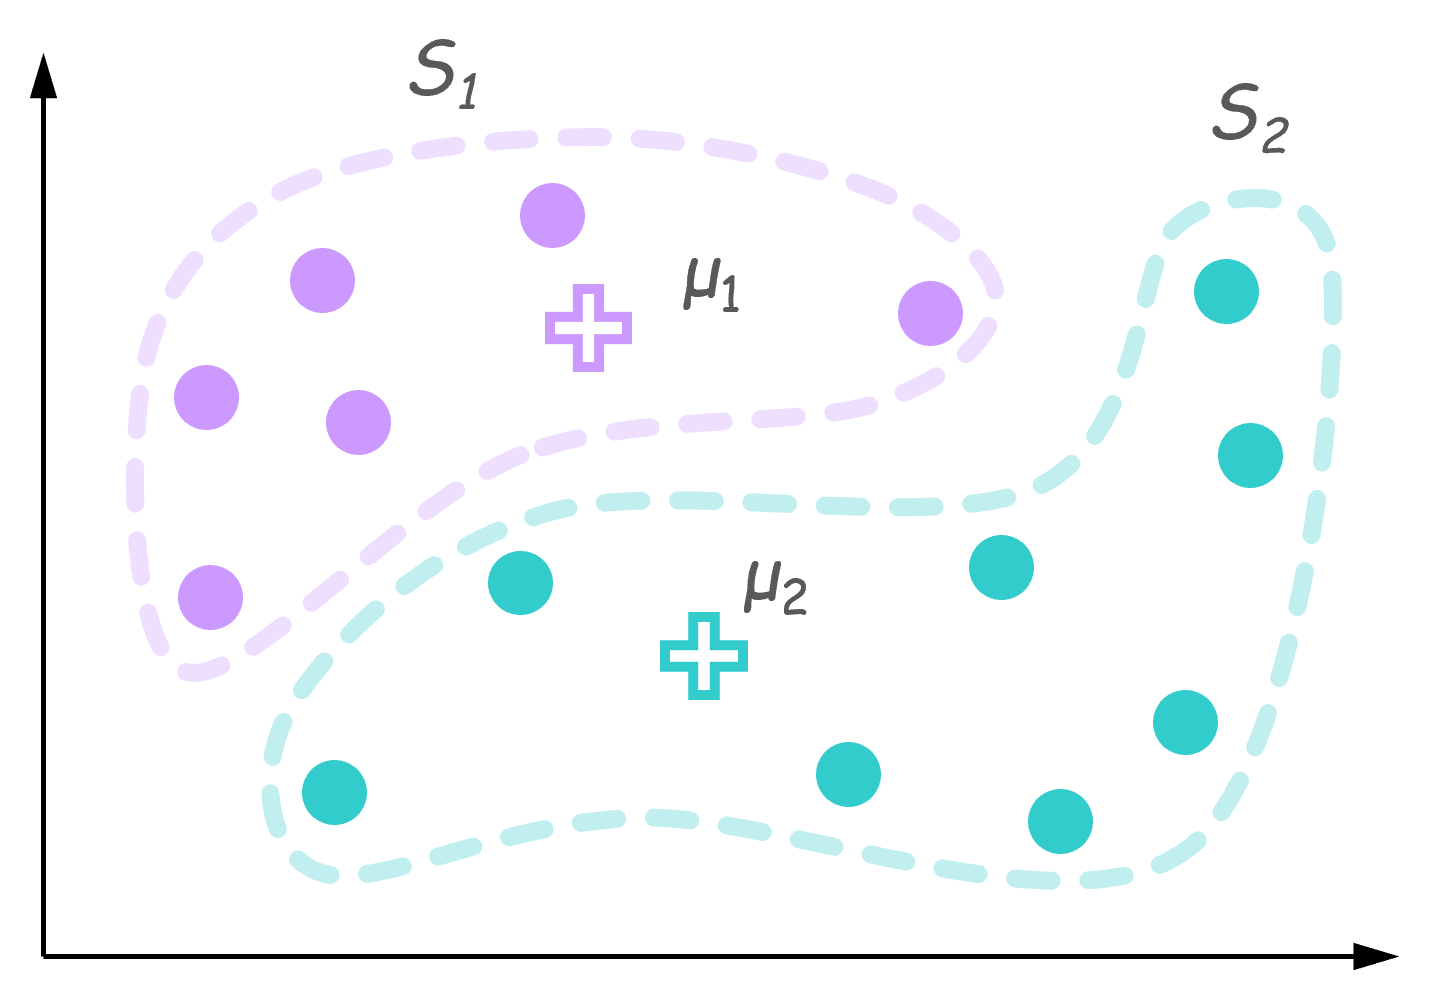
\includegraphics[width=2.2in]{./images/kClusterInitial.png}
            \caption{Initial cluster centroids}
        \end{minipage}
        \begin{minipage}[t]{0.45\textwidth}
            \centering
            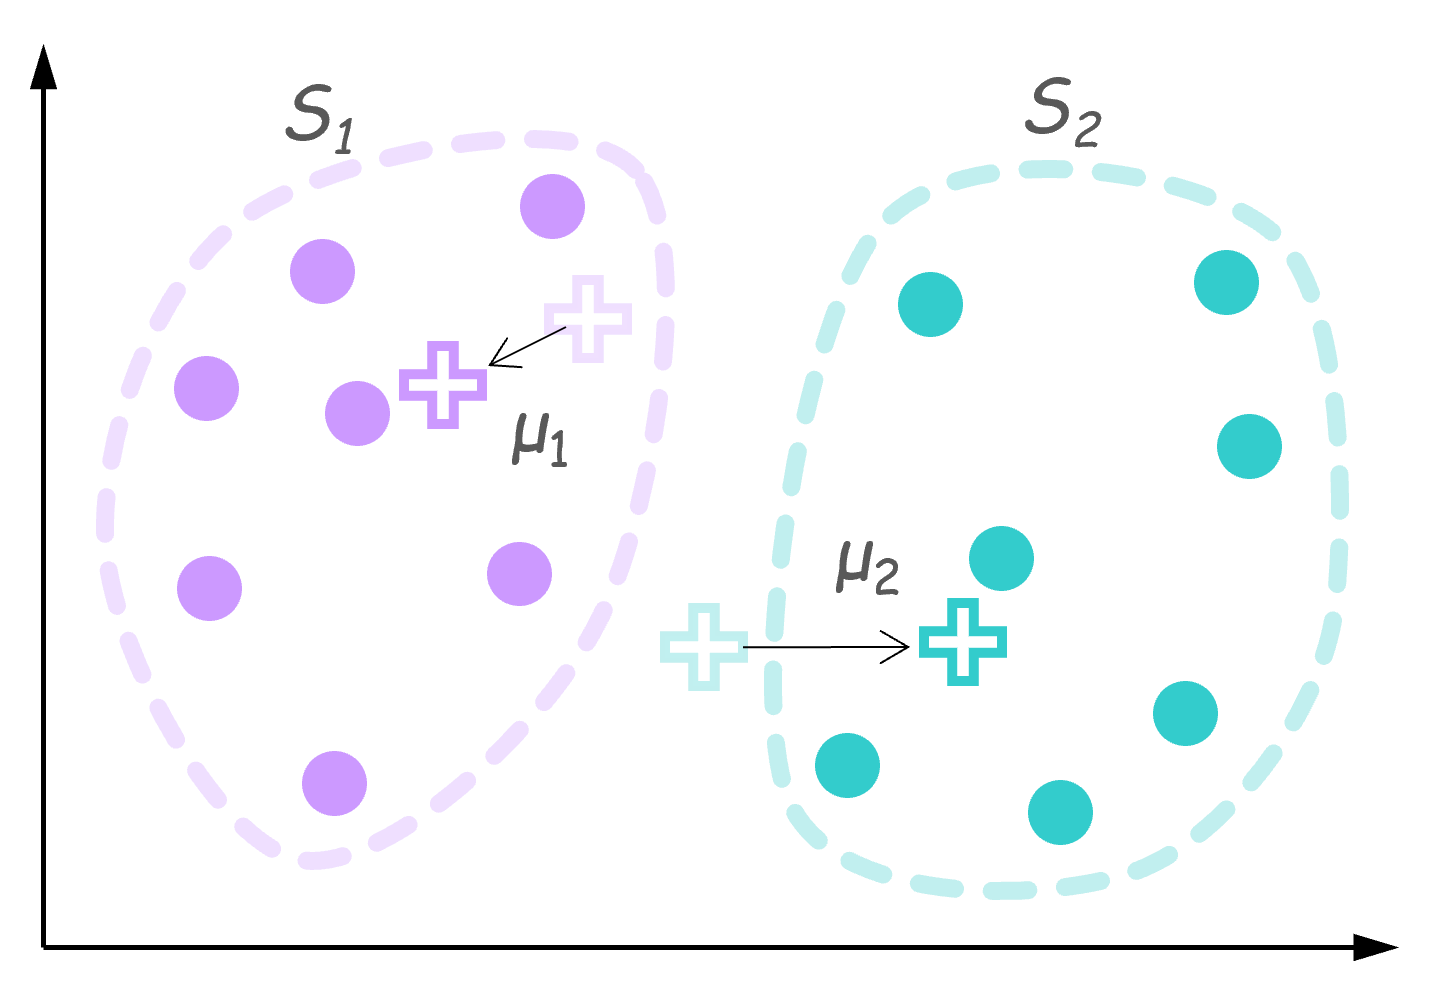
\includegraphics[width=2.2in]{./images/kClusterIter.png}
            \caption{Cluster centroids at first iteration}
        \end{minipage}
    \end{figure}
    
    \item Optimization objective
    \begin{equation}
        \mathop{\arg\min}\limits_{\textbf{S}} \sum_{k=1}^{K} \sum_{x^{(i)} \in S_i}\left\lVert {x^{(i)} - \mu_k} \right\rVert ^2
    \end{equation}
\end{itemize}


\section{Choosing the number of clusters}
\begin{itemize}
    \item Actually, there isn't a great way to choose the number of clusters automatically. 
    By far, the most common way is still choosing it manually by looking at visualizations or by looking at the output of the clustering algorithm.
    \item One common method is Elbow Method. The intuition is that increasing the number of clusters will naturally improve the fit.
    Once the line chart resembles an arm, then the ``elbow'' (the point of inflection on the curve) is a good indication that the underlying model fits best at that point.
    \begin{figure}[!htbp]
        \centering
        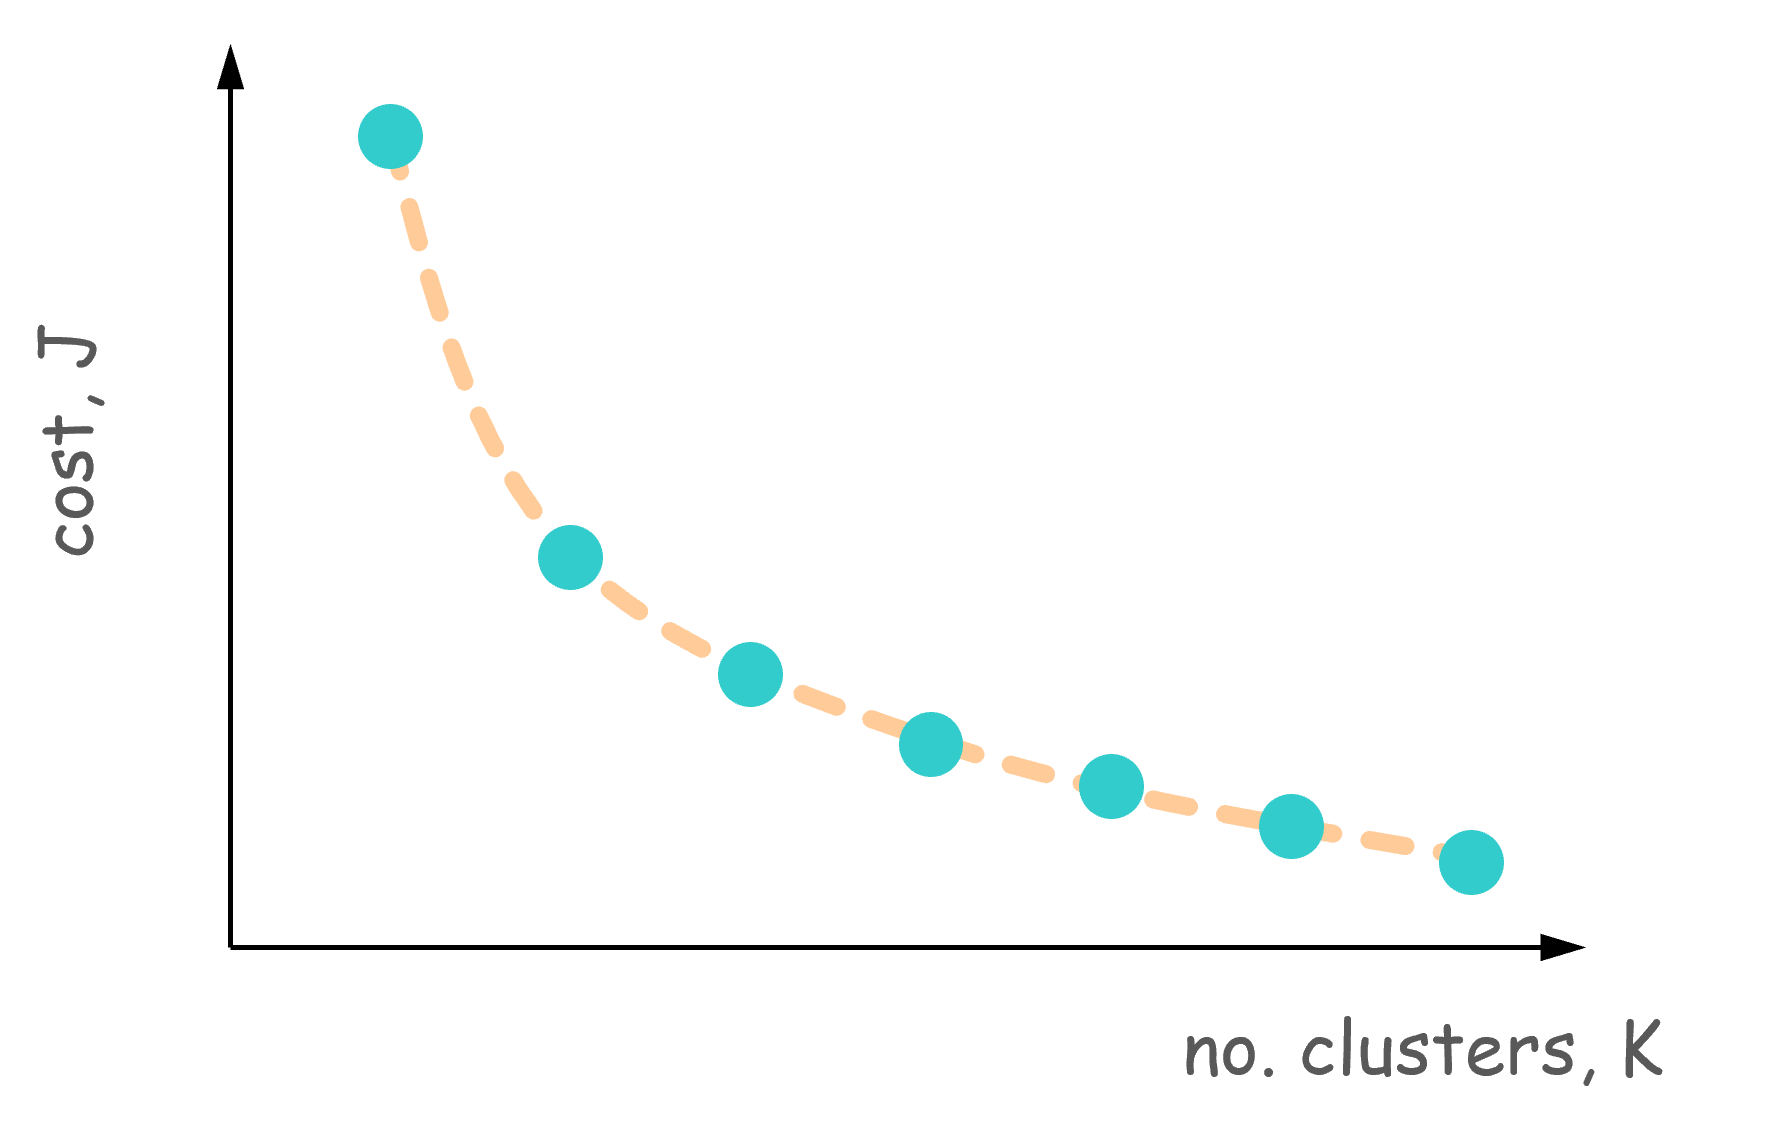
\includegraphics[width=3.2in]{./images/elbowMethod.png}
        \caption{The cost value differ with the number of clusters}
    \end{figure}
\end{itemize}
